\documentclass[10pt,a4paper]{report}
\usepackage[utf8]{inputenc}
\usepackage[english]{babel}
\usepackage{amsmath}
\usepackage{amsfonts}
\usepackage{amssymb}
\usepackage{graphicx}
\usepackage{hyperref}
\usepackage[autostyle, italian=quotes]{csquotes}
\usepackage[left=2cm,right=2cm,top=2cm,bottom=2cm]{geometry}
\author{Daniele Gilio}
\title{Assignment 4}
\begin{document}
\maketitle
\section{Introduction}
This assignment is about image classification. We are going to build a classifier that is able to distinguish between $12$ flower species. The dataset we will be working on contains $80$ images per species in the training set and $20$ per species in the test set.
\section{Data Augmentation}
Before passing to the actual classifiers description let us take a look at a very useful possibility in image recognition tasks. Working with images has a very positive element: \textit{Data Augmentation}. Since most features in images are independent from a lot of transformations (rotations, color saturation, image exposure, translation, etc.) we can expand a dataset by applying these transformations to it. Most of the times the bigger the dataset the better the performance. That said we are going to present our results with both the basic dataset and the augmented one.
\section{Low Level Classifier}
The first approach we tested was using a classifier that used \textit{Low Level Features}, which are specifically \enquote{crafted} functions that extract features from images. We tried using only one low level feature and then we tried using them all. With regards to the classifier we tested both a Single Layer Perceptron and a Multi Layer Perceptron. The first one had only the input layer, which dimensions matched the ones of the low level features, and the output layer made of $12$ neurons. The MLP had the same input layer than the sequence $[512, 128, 32, 12]$, representing the width of each subsequent layer.
\subsection{Single Feature}
The Single Feature strategy obtained a very low accuracy score. We choose to use the \textit{RGB Co-occurence Matrix} amongst all the possible ones because it was the best performing one. As we can see in Table \ref{tab:slf} the MLP got a much higher score as expected. Note that the augmented dataset increases considerably the performance of the networks. Both networks were trained for $500$ epochs with a batch size of $16$. The learning rate was set at $10^{-3}$ and was not modified during training.
\begin{table}[!ht]
\centering
\begin{tabular}{|l|c|c|}
\hline
                                   & SLP                        & MLP                        \\ \hline
Test Accuracy (Base) {[}\%{]}      & \multicolumn{1}{l|}{45.83} & \multicolumn{1}{l|}{60.83} \\ \hline
Test Accuracy (Augmented) {[}\%{]} & 60.83                      & 66.66                      \\ \hline
\end{tabular}
\caption{Single Low Feature Results}
\label{tab:slf}
\end{table}
\subsection{Multiple Features}
After the poor results obtained we decided to use all the available Low Level Features which are:
\begin{itemize}
\item Color Histogram
\item Edge Direction Histogram
\item Co-occurence Matrix
\item RGB Co-occurence Matrix
\end{itemize}
In order to use them together we just concatenated them in a big feature vector. The hyperparameters stayed the same for the MLP but we increased the epochs of training to $800$ for the SLP. This time the result were a bit better but we still consider them insufficient, as we can see in Table \ref{tab:mlf}. Anyway the significance of using the augmented dataset is once again proven.
\begin{table}[!ht]
\centering
\begin{tabular}{|l|c|c|}
\hline
                                   & SLP                         & MLP                         \\ \hline
Test Accuracy (Base) {[}\%{]}      & \multicolumn{1}{l|}{59.583} & \multicolumn{1}{l|}{69.583} \\ \hline
Test Accuracy (Augmented) {[}\%{]} & 71.25                       & 72.91                       \\ \hline
\end{tabular}
\caption{Multiple Low Features Results}
\label{tab:mlf}
\end{table}
\section{Neural Features} 
\subsection{PVMLNet as Feature Extractor}
A leap forward performance wise is to use a CNN (Convolutional Neural Network) as a feature extractor. This way the valuable features are autonomously learnt by the network. In order to do this we used a pre-trained network called \enquote{PVMLNet}, which structure we can see in Figure \ref{fig:pvmlnetstruct}.
\begin{figure}[!ht]
\centering
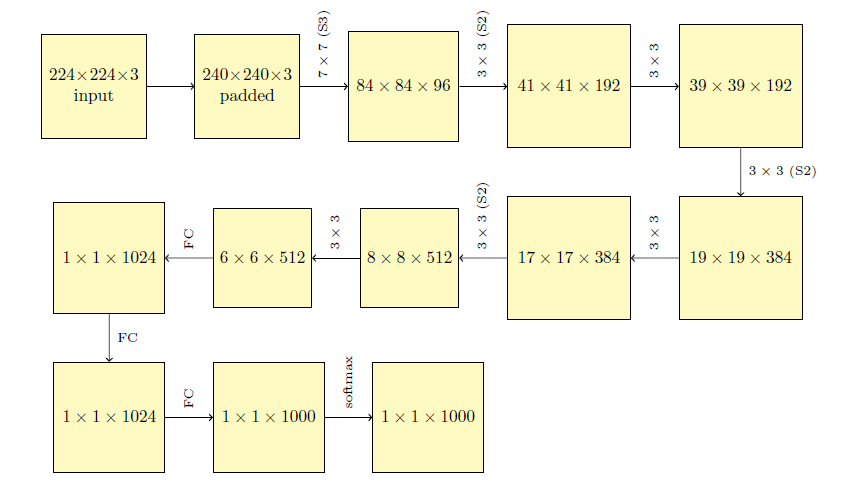
\includegraphics[width=0.75\linewidth]{pvmlnet.png}
\caption{PVMLNet Structure}
\label{fig:pvmlnetstruct}
\end{figure}
This network was trained on a subset of the ImageNet Dataset. This means that we are using the features that the network learnt on that dataset hoping that they are general enough to work on ours. To use PVMLNet as a feature extractor we need to remove at least the last two layers, and use the activations of the last remaining layer as the feature vector. We basically pass the each item in the dataset through the PVMLNet and record the activations of the last active layer as its features. Once we processed the whole dataset we train a SLP for the final classification. The first test was performed using the layer before the last two as the feature vector constructor (we will indicate this layer as $-3$, the last layer with this notation would than be $-1$ and the one before $-3$ would be $-4$). We then used layers $-4, -5$ and $-6$\footnote{Note that in order to use those layers we need to delete all the ones after them from PVMLNet and adjust the SLP input layer accordingly.}. We can see all this results in Table \ref{tab:ft-pvmlnet}. Note that we did not keep using the base dataset for all the tests we conducted, since we can be confident that using the augmented one is almost always the better choice.
\begin{table}[!ht]
\centering
\begin{tabular}{|l|c|c|c|c|}
\hline
                                   & Layer -3 & Layer -4 & Layer -5 & Layer -6 \\ \hline
Test Accuracy (Base) {[}\%{]}      & 88.75    & //       & //       & //       \\ \hline
Test Accuracy (Augmented) {[}\%{]} & 91.25    & 92.083   & 93.75    & 94.167   \\ \hline
\end{tabular}
\caption{PVMLNet Feature Extractor + SLP Results}
\label{tab:ft-pvmlnet}
\end{table}
The SLP was trained for $500$ epochs with a batch size of $50$. The learning rate was set at $10^{-3}$ and updated at each epoch\footnote{As always with update it with $\text{LR}=\text{LR}_0 \mathbin{/} \sqrt{t}$, where $t$ is the current epoch number.}. Table \ref{tab:ft-pvmlnet} seems to indicate that the further back we go into PVMLNet the better the result. We were not able to prove this result due to hardware limitations (we ran out of memory during layer $-7$ testing). Looking at Figure () we can see that we probably would have encountered the law of diminishing returns.
\subsection{Transfer Learning}
Another way to use PVMLNet as a feature extractor is via \textit{Transfer Learning}. This method consists in directly replacing the trained SLP to the removed layers in the CNN. This may seem unnecessary since this method yields the same results as the one described above. The major advantage of Transfer Learning is the possibility of \textit{Fine Tuning} the resulting network. This process is nothing but an additional training performed with a very low Learning Rate. The choice of this hyperparamter is crucial since in this case is very easy to fall into overfitting. We chose to fine tune our network for $25$ epochs, with a starting learning rate of $10^{-4}$. We needed to divide the training set in two, each epoch the network is trained on half the dataset in order to avoid memory limitations. Our results are presented in Table \ref{tab:ftft-pvmlnet}. We can clearly see that we had gained a little accuracy in the Layer $-3$, we slightly overfitted in Layer $-4$ case and we did not gain anything in Layer $-5$ and $-6$ cases. If we consider that the mean improvement was $0.079 \%$, fine tuning does not seem a very good idea for this problem with this dataset, or at least with the hyperparameters we used. 
\begin{table}[!ht]
\centering
\begin{tabular}{|l|c|c|c|c|}
\hline
                                   & Layer -3 & Layer -4 & Layer -5 & Layer -6 \\ \hline
Test Accuracy (Base) {[}\%{]}      & 89.167   & //       & //       & //       \\ \hline
Test Accuracy (Augmented) {[}\%{]} & 91.666   & 91.666   & 93.75    & 94.167   \\ \hline
\end{tabular}
\caption{Fine Tuned PVMLNet+SLP Results}
\label{tab:ftft-pvmlnet}
\end{table} 
\section{Results Analysis}
In order to better evaluate our network we computed the Confusion Matrices and annotated the image that was incorrectly classified with the most confidence. Since we did test multiple configuration we are going to discuss only the best classifier for each class, meaning SLP, MLP and Layer $-6$ networks trained on the augmented dataset. 
\begin{figure}[!ht]
\centering
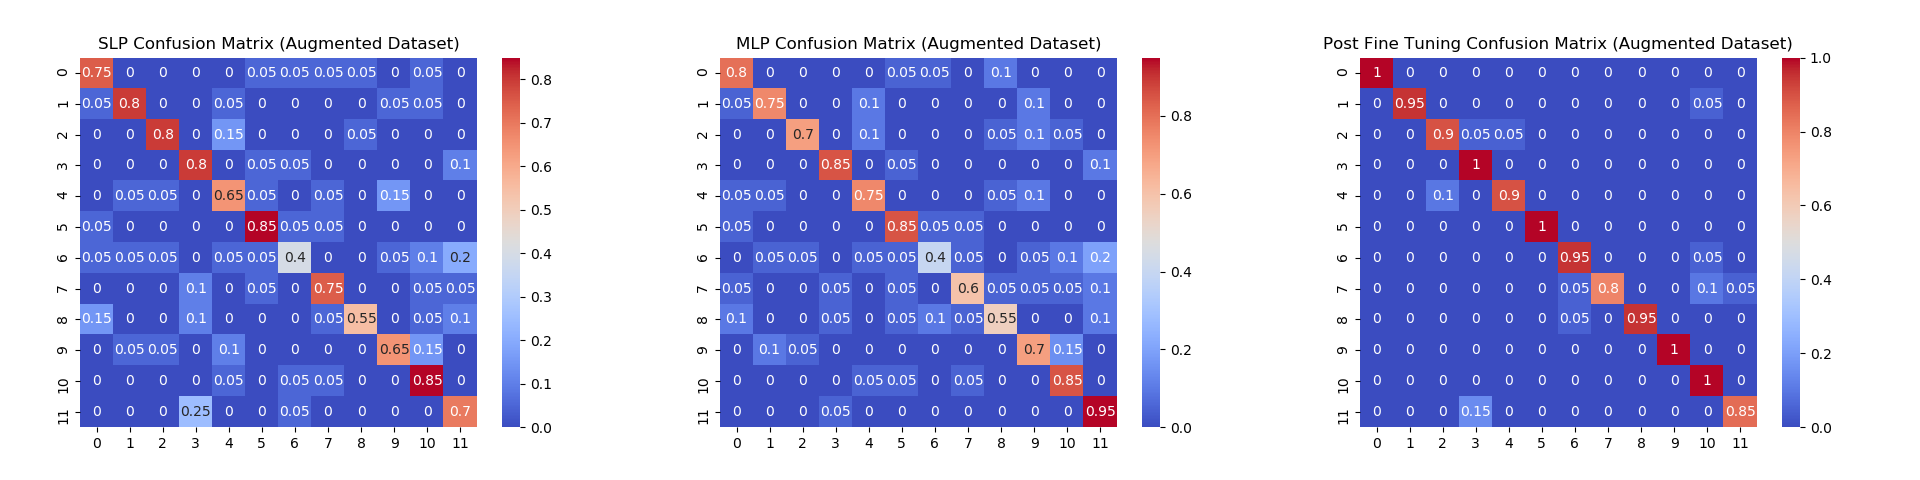
\includegraphics[width=\linewidth]{conf_mat.png}
\caption{Confusion Matrices: SLD (Left), MLP (Center) and Layer $-6$ (Right)}
\label{fig:confmat}
\end{figure} 
We can notice right away the performance gradient from left to right in Figure \ref{fig:confmat}. The SLP has a very noisy Confusion Matrix, Class $6$ (Iris) is the most misclassified one with an accuracy of only $40 \%$. The \enquote{most wrong} classification\footnote{image\_0425.jpg} is in fact an Iris (Class $6$) which is classified as a Windflower (Class $11$) with a confidence of $88.82 \%$. The image is easily distinguishable by a human. The MLP Matrix is less noisy but Class $6$ is still the less precise. That said though, the \enquote{wrongest} image\footnote{image\_1313.jpg} is a Pansy (Class $8$) classified as a Lily-Valley (Class $7$) with a confidence of $99.9963 \%$. Again, the image is completely distinguishable. As for the Level $-6$, we have most of the classes correctly classified. The less precise class is Lily-Valley (Class $7$), but the most misclassified image\footnote{image\_0884.jpg} is a Colts-Foot (Class $2$) classified as a Dandelion (Class $4$) with a confidence of $99.9999 \%$. Honestly speaking if we did not know that the image was a Colts-Foot we probably would have struggled to classify it. 
\section{Conclusions}
Based on the results we obtained, we can conclude that the Neural Features are the most effective. Letting a Network learn significant features by itself is the cleverest choice in this case. The SLP and MLP Networks greatly fall behind, achieving an accuracy of $30 \%$ less than the Layer $6$ case. The results obtained with Layer $6$ are not perfect, but still, we would not be able to outperform it without increasing our flower species knowledge. 
\vspace*{\fill}
\\
I affirm that this report is the result of my own work and that I did not share any part of it with anyone else except the teacher.
\\
\end{document}